\chapter{软件补丁兼容性检测方法}
\section{兼容性问题}
\label {define_problem}
第一章中对本文所要解决的问题进行了简要介绍。下面对该问题进行正式的定义。

%\begin{problem}
%	\label {origin}
	针对某软件系统s,假设已有版本$v_1$和$v_2$,其中补丁$p_1$是针对版本$v_1$而设计,应用后能使其演进到版本$v_3$,问$p_1$是否能够应用于版本$v_{2}$,并且应用之后是否会发生冲突?
%\end{problem}

考虑到补丁间不兼容的实质是因为在应用时和应用后出现了错误,可以具体将错误分为两类:

\begin{definition}
	兼容性错误——将补丁$p_1$和补丁$p_2$先后应用于同一版本代码$v$时和之后所出现的程序错误。主要分为两类:
	\begin{itemize}
		\item 语法错误:即在应用一补丁$p_1$之后,再次应用另一补丁$p_2$时出现语法结构上的错误。
		\item 语义错误:将补丁$p_1$中的变更和补丁$p_2$中的变更应用于源代码之后,由于语义上的变更互相冲突而导致出现了功能上的错误
	\end{itemize}
\end{definition}

其中,语法错误易由编译器发现,而语义错误深藏于代码中,较难发现。可见,该问题的核心包括两点,即:
\begin{itemize}
	\item 如何将一个专为版本$v_1$设计的补丁$p_1$成功应用于版本$v_2$上。即如何消去补丁应用过程中的语法错误。
	\item 如何检测补丁在应用于新版本之后是否会与该版本代码产生冲突?即如何检测补丁应用之后的语义错误。
\end{itemize}

下面分别对这两点进行分析和阐述。

\subsection{补丁应用}

实际上,补丁程序是专门为某一版本的软件系统所设计,因而往往不能直接应用到其他版本的代码上,而且强行应用往往会出现很多错误。常见的问题可能包括:

\begin{enumerate}
	\item 补丁程序中所提及的行不在原位置。
	\item 补丁程序中所要删除的行其实已被删除,或者所要添加的行其实已被添加。
	\item 补丁程序中所提及的文件未找到。
\end{enumerate}

由于有这些可能的问题存在,导致我们无法直接将补丁程序应用到其他版本的补丁上。因此,我们考虑如何去解决问题的第一点:

由于补丁$p_1$针对版本$v_{1}$设计,当尝试将其应用到版本$v_{2}$上时,可能会出现程序语法结构上的错误,考虑怎样将$p_1$成功应用到版本$v_{2}$上,使得该过程不会引入程序语法错误。

%\begin{problem}
%	\label {patch_reversion}
	
%\end{problem}

	假若用$Code$表示源代码,$Patch$表示补丁,即变更的集合。用$patch(p,v)$函数表示将补丁$p$应用于版本$v$的过程。用$Pat$函数判断某个补丁是否适用于某个版本的代码。用$error$函数表示对源代码的语法检查,其结果表明源代码中是否存在语法错误。其中$v_k$表示代码的第k个版本,$p_i$表示第i个补丁。
	
	那么我们可以将其定义如下:
\begin{definition}
	给定$p_i$,$v_k$,问$p_i \not \subset Pat(v_k)$时,能否使得$error(patch(p_i,v_k)) == False$?其中$p_i \subset Patch,v_k \subset Code,i,k \subset \mathbb{N}$。
\end{definition}
	
	

%\begin{definition}
%	$patch: Patch \times Code \mapsto Code$。$patch(p_i,v_k) = v_m,v_k,v_m \subset Code,i,k,m \subset \mathbb{N}$。
%\end{definition}

%\begin{definition}
%	$Pat: Code \mapsto \{Patch\}$。用于表示代码到其对应的补丁集合的映射,可用于判断某个补丁是否适用于某个版本的代码。
%\end{definition}

%\begin{definition}
%	$error: Code \mapsto Boolean$。error函数用于对源代码的语法检查,其结果表明源代码中是否存在语法错误。
%\end{definition}

%\begin{definition}
%	\label {app_formal}

%\end{definition}

可见,要解决问题的第一点,其核心在于如何给出合适的$patch(p_i,v_k)$函数,使得$p_i$应用于版本$v_k$之后不会出现语法错误。

考虑到$patch(p_1,v_1) = v_3$,为了将$p_1$应用到版本$v_2$上获得版本$v_4$,我们可以采用某种归并算法,将版本$v_3$和版本$v_2$进行合并即可。合并后我们就等于同时拥有了$p_1 = diff(v_1,v_3)$和$p_2 = diff(v_1,v_2)$这两个补丁中的变更。

整个过程可以形式化定义如下。实际上也就是说我们用$merge$函数实现了将补丁应用于其他版本的代码的功能。

\begin{definition}
	$merge: Code \times Code \mapsto Code$。$v_s = patch(p_i,v_l) = merge(v_m,v_l)$,使得$\forall c_a \subset p_i,\forall c_b \subset p_j,c_a,c_b \subset p_k$,即$p_k = p_i \cup p_j$。其中$v_m = patch(p_i,v_n),p_j = diff(v_n,v_l),p_k = diff(v_l,v_s),p_i \not \subset Pat(v_l),p_i,p_j \subset Pat(v_n),p_k \subset Pat(v_l),v_l,v_m,v_n,v_s \subset Code,a,b,i,j,k,l,m,n,s \subset \mathbb{N}$。
\end{definition}

\subsection{补丁冲突}

就问题的第二点而言,直接去寻找冲突的存在是一件让人困惑的事情,什么是冲突?为什么会发生冲突?怎么进行检测?

因此本文考虑从另一个角度来看待这一点。

实际上,由于从版本$v_1$到版本$v_2$的演进过程同样可以使用补丁来完成。那么可以考虑将这个演进过程表述成为使用补丁进行变更的过程,以得到另外一个用于进行版本更新的补丁。

\begin{definition}
	\label {define_diff}
	$diff : Code \times Code \mapsto Patch$。其中$p = diff(v_i,v_j) \iff patch(p,v_i) = v_j,i,j \subset \mathbb{N},p \subset Pat(v_i)$。该函数用于求解两个不同版本的程序$v_i$和$v_j$之间的差异性,其结果即为补丁p。
\end{definition}

从问题中可以发现,$p_{1} = diff(v_{1},v_{3})$。如果同样给定$p_{2} = diff(v_{1},v_{2})$,并且问题的第一点已经得到了妥善的解决,那么,对于问题的第二点而言,如何检测补丁在应用于新版本之后是否会与该版本代码产生冲突就可以规约如下:

%\begin{problem}
%	\label {compatible}
	给定针对某同一版本代码$v$的补丁$p_1$和$p_2$,问分别应用于$v$之后,这两个补丁对于该版本代码的语义影响是否会产生冲突?
%\end{problem}

这样一来,问题的实质就清楚了。显然,该问题是由于两个补丁同时对同一版本代码造成了语义影响而引起的。那么为了回答这个问题,我们需要明确的知道到底什么是补丁对代码的语义影响,以及什么是冲突。

本文首先讨论什么是补丁对代码的语义影响。

语义影响(Semantic Impact)是由于代码之间存在着某种依赖关系而造成的,因此假如某个代码结构对其他代码结构存在依赖关系,那么就说这两者间存在语义影响。其中代码结构指程序的语法结构,包括类、方法、语句等不同的类型。

%\begin{definition}
%	
%\end{definition}

事实上,如果给出不同的依赖关系的定义,那么就会得到不同类型的影响。可见,这里所谓的语义影响即是程序代码间的耦合关系。常见的依赖关系包括控制依赖和数据依赖等。

下面给出语义影响的定义。其中Structure用于表示程序代码结构,Sturct函数为从源代码到其所有代码结构集合的映射。其中依赖关系可以包括控制依赖、数据依赖等。

%\begin{definition}
%	$Structure \to Class \mid Method \mid Statement \mid ...$。Structure用于表示程序代码结构,可以任意替换为对应的子类型。
%\end{definition}

%\begin{definition}
%	$Struct: Code \mapsto \{ Structure \}$。
%\end{definition}

\begin{definition}
	$im: Structure \mapsto Structure$。影响关系定义为一个从代码结构到代码结构的映射关系,$im(structure_i) = structure_j$用于表示代码结构$structure_i$受到$structure_j$影响,$i,j \subset \mathbb{N}$。
\end{definition}

\begin{definition}
	$depend: Structure \mapsto Structure$。依赖关系定义为一个从代码结构到代码结构的映射关系,$depend(structure_i) = structure_j$用于表示代码结构$structure_i$依赖于$structure_j$,$i,j \subset \mathbb{N}$。
\end{definition}

\begin{definition}
	$\forall structure_i,structure_j \subset Struct(v_k),  im(structure_i) = structure_j \iff depend(structure_i) = structure_j$,其中$v_k \subset Code,i,j,k \subset \mathbb{N}$。
\end{definition}

从中可见代码结构$structure_i$受到$structure_j$的影响,当且仅当代码结构$structure_i$依赖于$structure_j$。


%\begin{definition}
%	\label {define_conflict}
%
%\end{definition}

因此,可以认为,语义冲突(Confilict)是指两个补丁所对应的不同变更集合之间存在某两条互斥的变更,其中两条变更互斥指二者的语义互相影响。

若$change$函数用于表示代码结构和其所对应的变更的映射,那么可以将其定义如下。

%\begin{definition}
%	
%\end{definition}

%\begin{definition}
%	$change: Structure \mapsto Change$。用于表示代码结构和其所对应的变更的映射。其中$Change$——指变更。$Patch = \{Change\}$。
%\end{definition}


\begin{definition}
	$conflict: Patch \times Patch \mapsto Boolean$。如果$\exists structure_i,structure_j,structure_k \subset v_t$,使得$im(structure_i) = structure_k \land im(structure_j) = structure_k$,那么$conflict(p_m,p_n) = True$。其中$change(structure_i) \subset p_m,change(structure_j) \subset p_n,p_m,p_n \subset Pat(v_t),v_t \subset Code,i,j,k,m,n,t \subset \mathbb{N}$。
\end{definition}

该$confilct$函数用于判断两个补丁是否发生语义冲突。该函数表示,假如补丁$p_m$中的某条变更修改了代码结构$structure_j$,补丁$p_n$中的某条变更修改了代码结构$structure_i$,并且代码结构$structure_i$和$structure_j$影响到了同一个代码结构$structure_k$,那么就说明补丁$p_n$和$p_m$之间存在着语义冲突。

在有了语义影响和冲突的定义之后,问题的第二点就可以形式化的描述如下:

%\begin{problem}
%	\label {compatible_formal}
	给定$v_k \subset Code, p_i,p_j \subset Pat(v_k),i,j,k \subset \mathbb{N}$,问是否有$conflict(p_i,p_j) == True$?
%\end{problem}

%因此,结合前文中对问题第一点的形式化描述,该问题就可以形式化的定义如下:
%
%%\begin{problem}
%%	\label {origin_formal}
%	给定$p_i,v_k,v_m$,问当$p_i \not \subset Pat(v_k)$时,如果能够使得$compile(patch(p_i,v_k)) == True$,并且$\exists p_j = diff(v_k,v_m)$,那么是否有$conflict(p_i,p_j) == True$?其中$p_i \subset Patch,p_j \subset Pat(v_k),v_k,v_m \subset Code,i,j,k,m \subset \mathbb{N}$。
%%\end{problem}

%\section{问题分析}
%\label {problem_analysis}
%
%\subsection{补丁应用}
%\label {patch_app}

%如前所述,为了解决问题的第一点,主要需要提供合适的$patch(p_i,v_k)$函数。

%实际上可以采用版本控制系统的版本合并功能来作为该函数的具体实现。
%
%版本控制系统中经常需要将其他分支中的版本合并到当前分支中,为了解决不同版本之间可能存在的语法冲突,通常会采用三路归并算法(3-way merge)来对两个不同版本的代码进行合并,合并时以二者共同的祖先版本作为依据进行。



%这实际上也是现在软件开发过程中的常见手段。例如使用git作为版本控制系统时,为了修复某个功能性的bug,我们可以新建一个分支FixBug,然后切换到该分支进行漏洞修复,等到修补完毕后,再将该分支合并到主分支Master中即可。
%
%该过程如图\ref{git_branch}所示。
%
%\begin{figure}[H]	
%	\centering
%	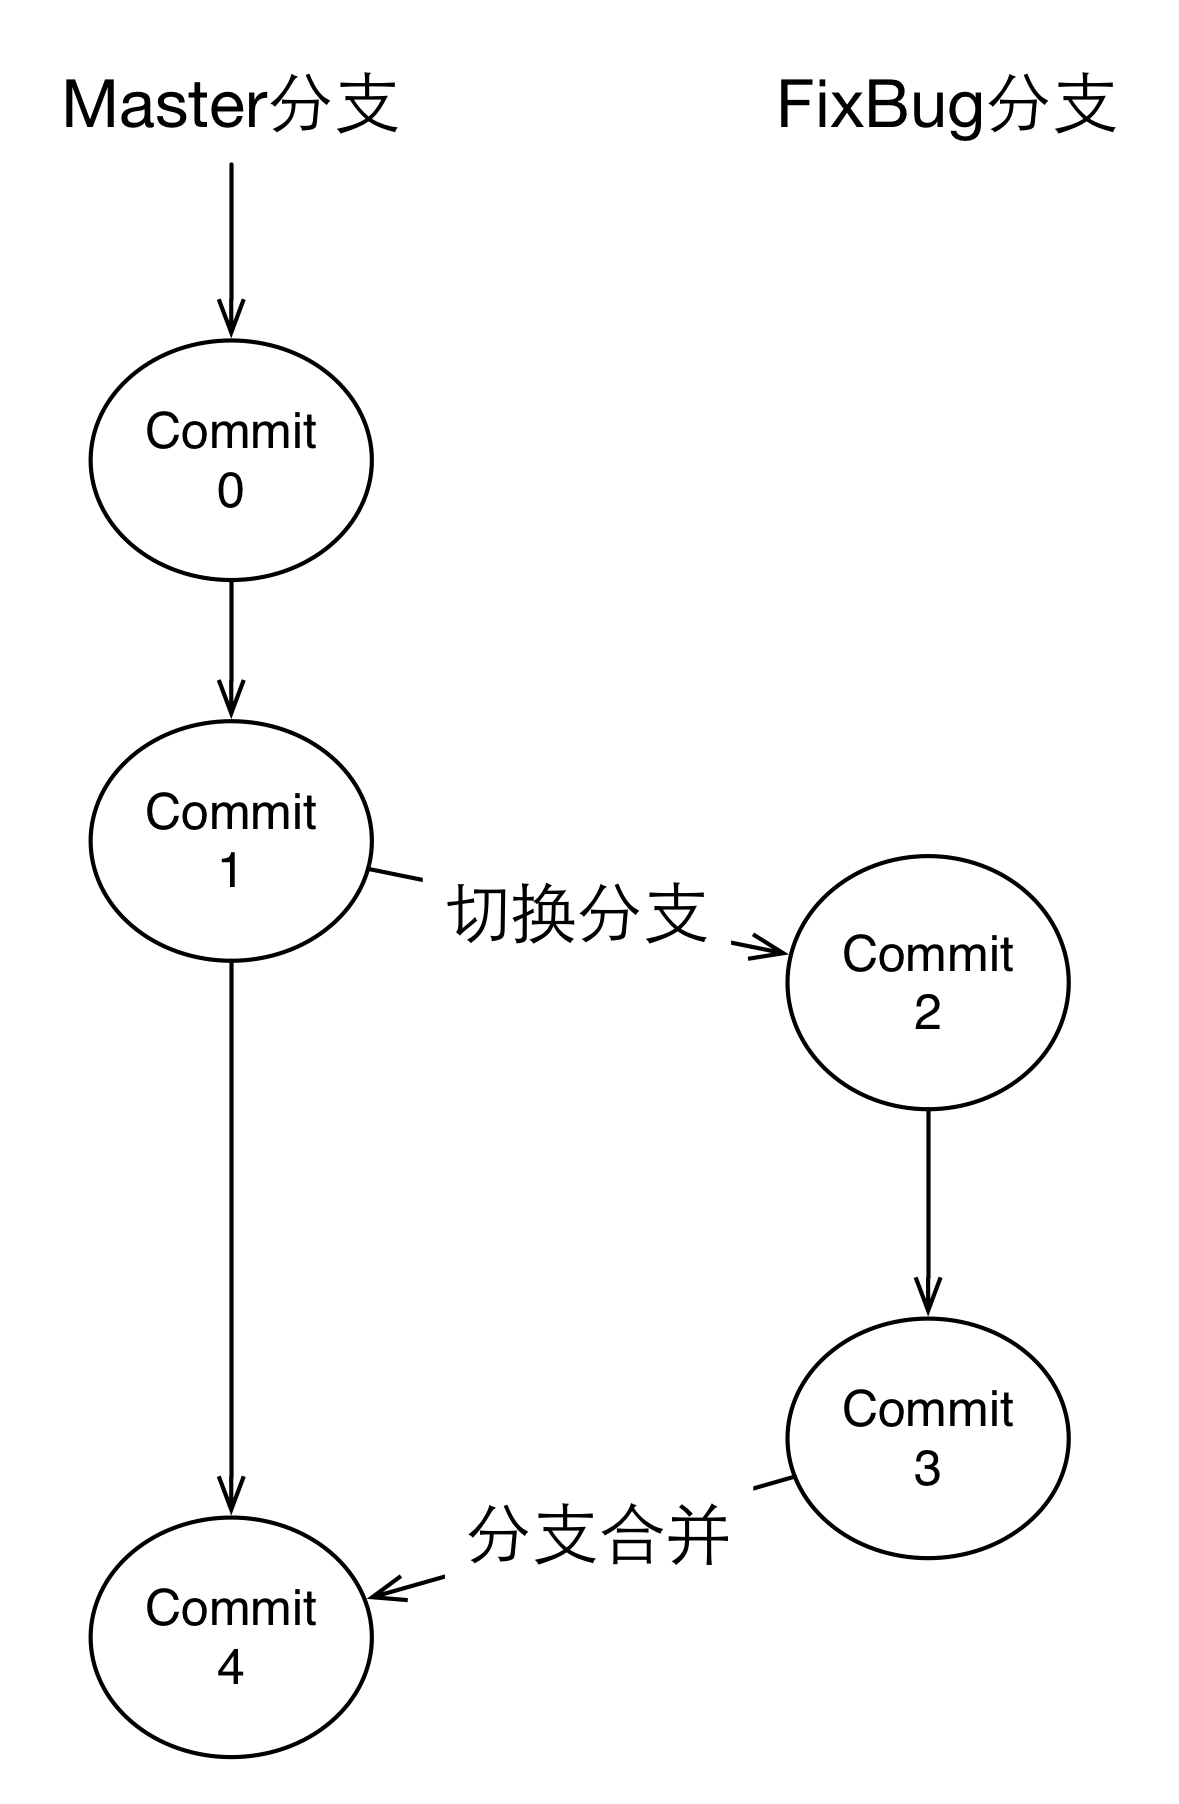
\includegraphics[height=.6\columnwidth]{chap03_git_branch}
%	\caption {git分支切换与合并}	
%	\label {git_branch}
%\end{figure}


%\subsection{补丁冲突}
%\label {conflict}

为了解决问题的第二点,我们主要需要从代码中挖掘中两类信息:
\begin{enumerate}
	\item 代码的变更集合,即两个版本之间代码的差异性。用于进行问题规约。
	\item 变更的影响集合,即变更集合对代码中其他哪些部分会造成影响。用于确定变更造成的语义影响。
\end{enumerate}

在有了这两类集合之后,我们就可以界定出软件变更在语义层面上对代码的语义影响域,我们可以将这整个过程称为语义影响域分析(Semantic Impacted Area Analysis)。

下面首先给出语义影响域的概念。语义影响域(Sematic Impated Area)是指程序的某个限定范围中,直接或间接受到变更影响的程序结构集合。其中程序结构——指程序的基础语法结构,包括类、方法、基本块、语句等不同级别。

%\begin{definition}
%	
%\end{definition}
%
%\begin{definition}
%	
%\end{definition}

可见,语义影响域描述了变更对于程序中其他部分的语义影响。下面给出影响域的定义。

\begin{definition}
	$impact: Patch \times Code \mapsto \{Structure\}$。$impact(p_m, v_k) = \{ \forall structure_j \subset Struct(v_k) \mid structure_j = im(sturcture_i) \land (change(structure_i) \subset p_m \lor structure_i \subset impact(p_m,v_k)),structure_i,structure_j \subset Struct(v_k),v_k \subset Code,p_m \subset Pat(v_k), i,j,k,m \subset \mathbb{N} \}$。
\end{definition}

该函数用于描述补丁$p_m$对于其所应用的某个版本的代码$v_k$的影响域。其中可以将影响关系$im$限定在不同代码结构类型的范围内。

为了挖掘出这两类信息,可以将语义影响域分析划分为两个子过程:
\begin{enumerate}
	\item 程序间差异性分析:获取两个软件版本间的差异性,获得结构化的软件变更信息。该分析过程即为$diff$函数的具体实现。
	\item 变更影响分析:分析软件变更对软件其他部分是否存在影响,并找到受影响的集合。该分析过程即为$impact$函数的具体实现。
\end{enumerate}



在有了软件变更的语义影响域之后,我们可以通过简单地比较两个补丁对代码的影响域是否存在重叠来判定其是否发生了语义冲突。语义冲突(Semantic Confilict)的实质就是指两个补丁所对应的不同变更集合之间存在某两条互斥的变更。其中两条变更互斥指二者对同一行代码进行了修改,或者他们所修改了不同行代码,但其影响传播到了某行相同的代码。

%\begin{definition}
%	\label {define_conflict}
%	
%\end{definition}

%为了更清楚的理解,可以给出如下的形式化定义。
%也就是说:
%\begin{definition}
%	\label {problem}

%	如果$\exists c_m \subset p_i, \exists c_n \subset p_j$,其中$c_m = change(structure_m),c_n = change(structure_n)$, $structure_m \subset Struct(v_k), structure_n \subset Struct(v_k), v_k \subset Code$,并且$i,j,k,m,n \subset \mathbb{N}$。
%	那么有$conflict(p_i,p_j) == true \iff (structure_m == structure_n) \lor (impact(p_i,v_k) \cap impact(p_j,v_k) \neq \varnothing)$,其中$p_i,p_j \subset Pat(v_k)$。
%\end{definition}

可见,如果两个补丁对代码的影响域不存在重叠,那么他们两者之间自然是兼容的,因为他们不仅本身的变更互不干涉,并且他们所影响到的程序结构也互不干涉。在这样的情况下,补丁是可以成功应用到其他版本上的代码,并且可以完成补丁本身的目标的。

如果影响域发生了重叠,那么我们就可以认为补丁之间是可能不相容的,因为补丁所作的变更会对相同的程序结构产生影响。而该部分代码是否发生冲突了还需要人工的判定,因为在不同的场景下,他们可能是兼容的,也可能是不兼容的。而我们无法从代码中获取到足够的信息来进行这样的判定,需要外界对于变更的期望信息作为辅助。

%我们可以将这个过程定义为如下类型的函数,并称之为冲突分析。可见,我们实际上是采用了$isCompatible(s_i,s_j)$函数来作为$conflict(p_i,p_j)$的具体实现。
%
%\begin{definition}
%	$isCompatible(s_i,s_j) : 、\{Structure\} \times \{Structure\} \mapsto Boolean$。其中$conflict(p_i,p_j) = isCompatible(impact(p_i,v_i),impact(p_j,v_j)),i,j \subset \mathbb{N}$。
%\end{definition}

\subsection{总结}

根据前两节中对问题各点的分析,可以得到对该问题的形式化描述:

给定$p_i,v_k,v_m$,问当$p_i \not \subset Pat(v_k)$时,如果能够使得$error(patch(p_i,v_k)) == False$,并且$\exists p_j = diff(v_k,v_m)$,那么是否有$conflict(p_i,p_j) == True$?其中$p_i \subset Patch,p_j \subset Pat(v_k),v_k,v_m \subset Code,i,j,k,m \subset \mathbb{N}$。


可以发现,对于整个问题而言,其解决方法的核心在于:
\begin{itemize}
	\item 如何将补丁成功应用于其他版本?即$merge$函数的具体实现。
	\item 如何检测补丁间的冲突?该部分的解决过程可以分为两步:
	\begin{enumerate}
		\item 如何规约该问题并计算影响域?即$diff$和即$impact$函数的具体实现。也就是整个语义影响域分析的过程。
		\item 如何判定发生了冲突?即$conflict$函数的实现。也就是整个冲突分析的过程。		
	\end{enumerate}
\end{itemize}

因此,整个补丁兼容性问题实际上可以归结为多次软件变更的影响域冲突检测问题。


\section{检测方法}
\label {problem_solve}

考虑前一节中对问题的定义与分析,我们可以给出一个通用的解决方案来解决整个补丁兼容性问题。

\subsection{整体架构}
\label {problem_all}

根据前文中的问题分析,实际上整个兼容性问题的解决过程可以参考图\ref {all_flow}。其输入输出的描述参考表\ref {all_io}。

可见,整个解决方案的实现过程包括三步:
\begin{itemize}
	\item 补丁应用过程。将专为某版本代码而设计的补丁应用于其他版本的代码,即$merge$函数的实现过程。
	\item 软件变更影响域分析过程。分析补丁中的变更所造成的语义影响,即$diff$函数和$impact$函数的实现过程。
	\item 软件变更冲突检测过程。检测补丁间的变更其影响域是否会发生冲突,即$conflict$函数的实现过程。
\end{itemize}

\begin{figure}[H]
	\centering
	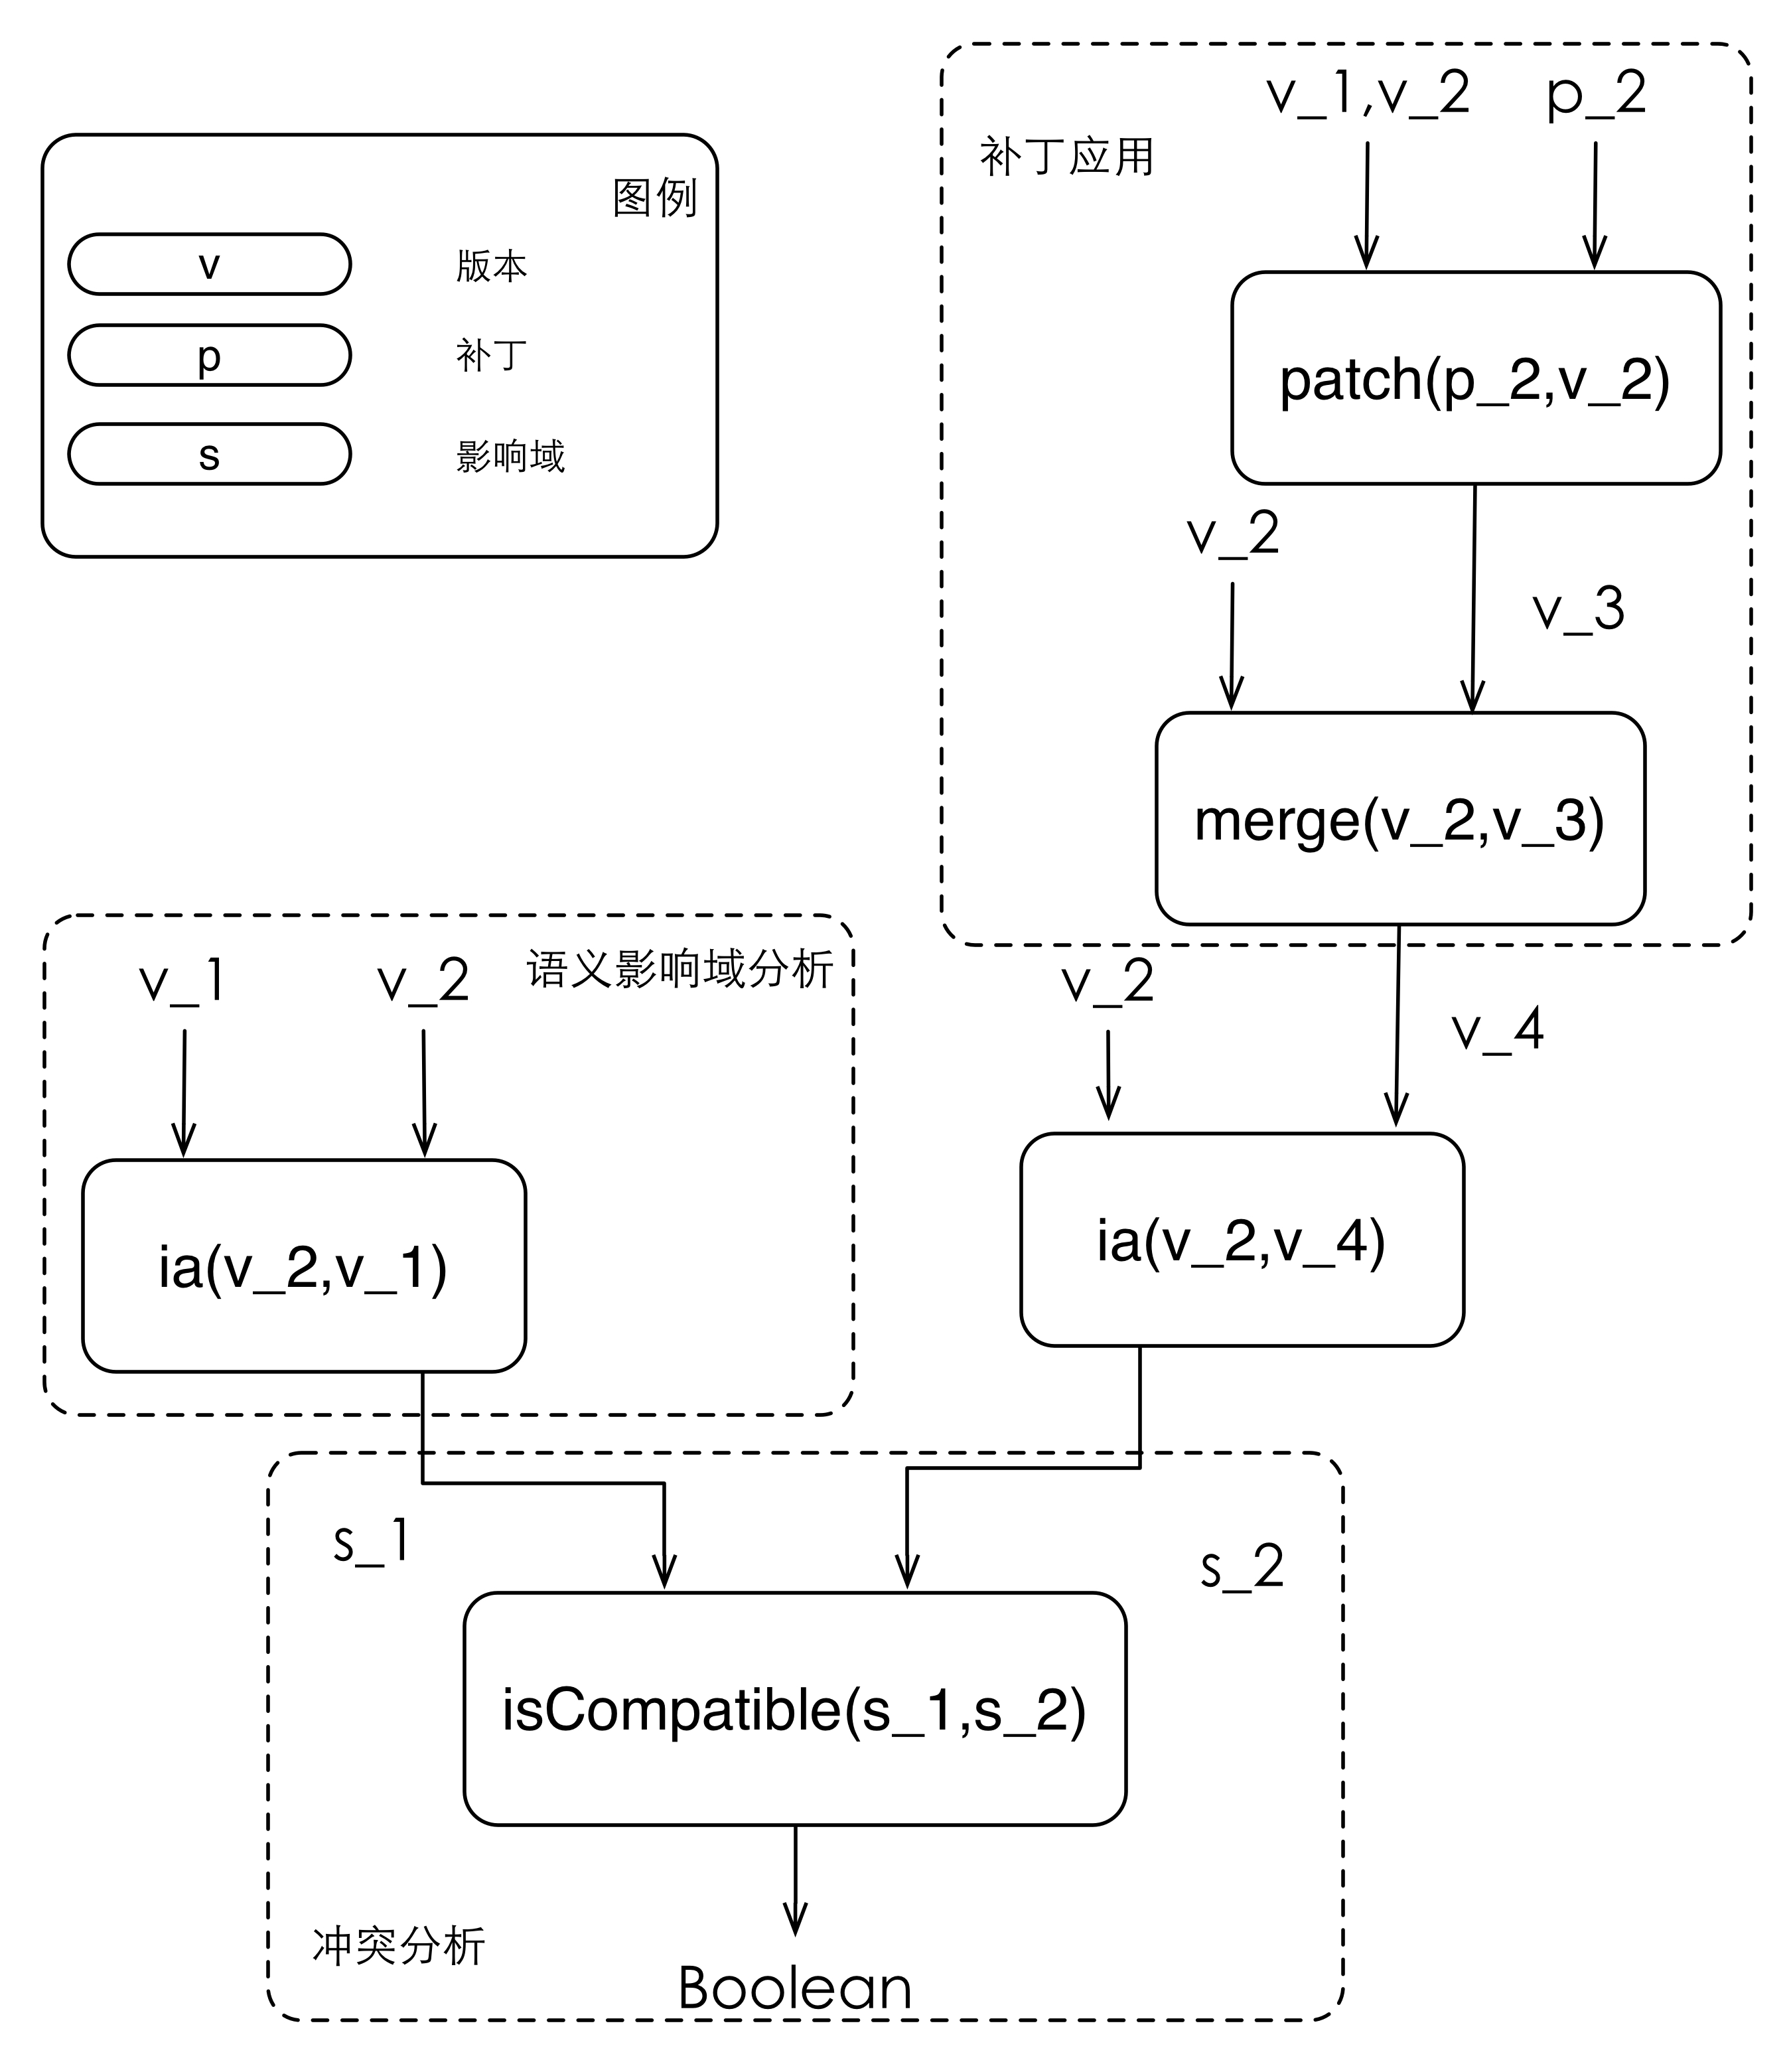
\includegraphics[height=.6\columnwidth]{chap03_all_flow_2}
	\caption {解决方案}
	\label {all_flow}	
\end{figure}

\begin{table}[H]
	\caption{输入输出对照表}
	\label{all_io}
	\centering
	\begin{tabular}{lc}
		\toprule[1.5pt]
		{\heiti 输入输出} & {\heiti 描述}\\\midrule[1pt]
		$v_1$ & 旧版本源代码,待检测的对象 \\
		$v_2$ & 新版本源代码 \\
%		$v_3$ & 将补丁$p_2$应用于版本$v_2$后的源代码 \\
		$v_4$ & 将补丁$p_2$中的变更应用于版本$v_1$后的源代码 \\
		$p_2$ & 适用于$v_2$的补丁,待检测的对象 \\
		$s_1$ & $diff(v_2,v_1)$对版本$v_2$的影响域 \\
		$s_2$ & $diff(v_2,v_4)$对版本$v_2$的影响域 \\
		结果 & 是否冲突 \\
		\bottomrule[1.5pt]
	\end{tabular}
\end{table}

因此,实现该补丁兼容性检测方法的工具可以设计成如图\ref {structure}所示的组合形式。

\begin{figure}[H]
	\centering
	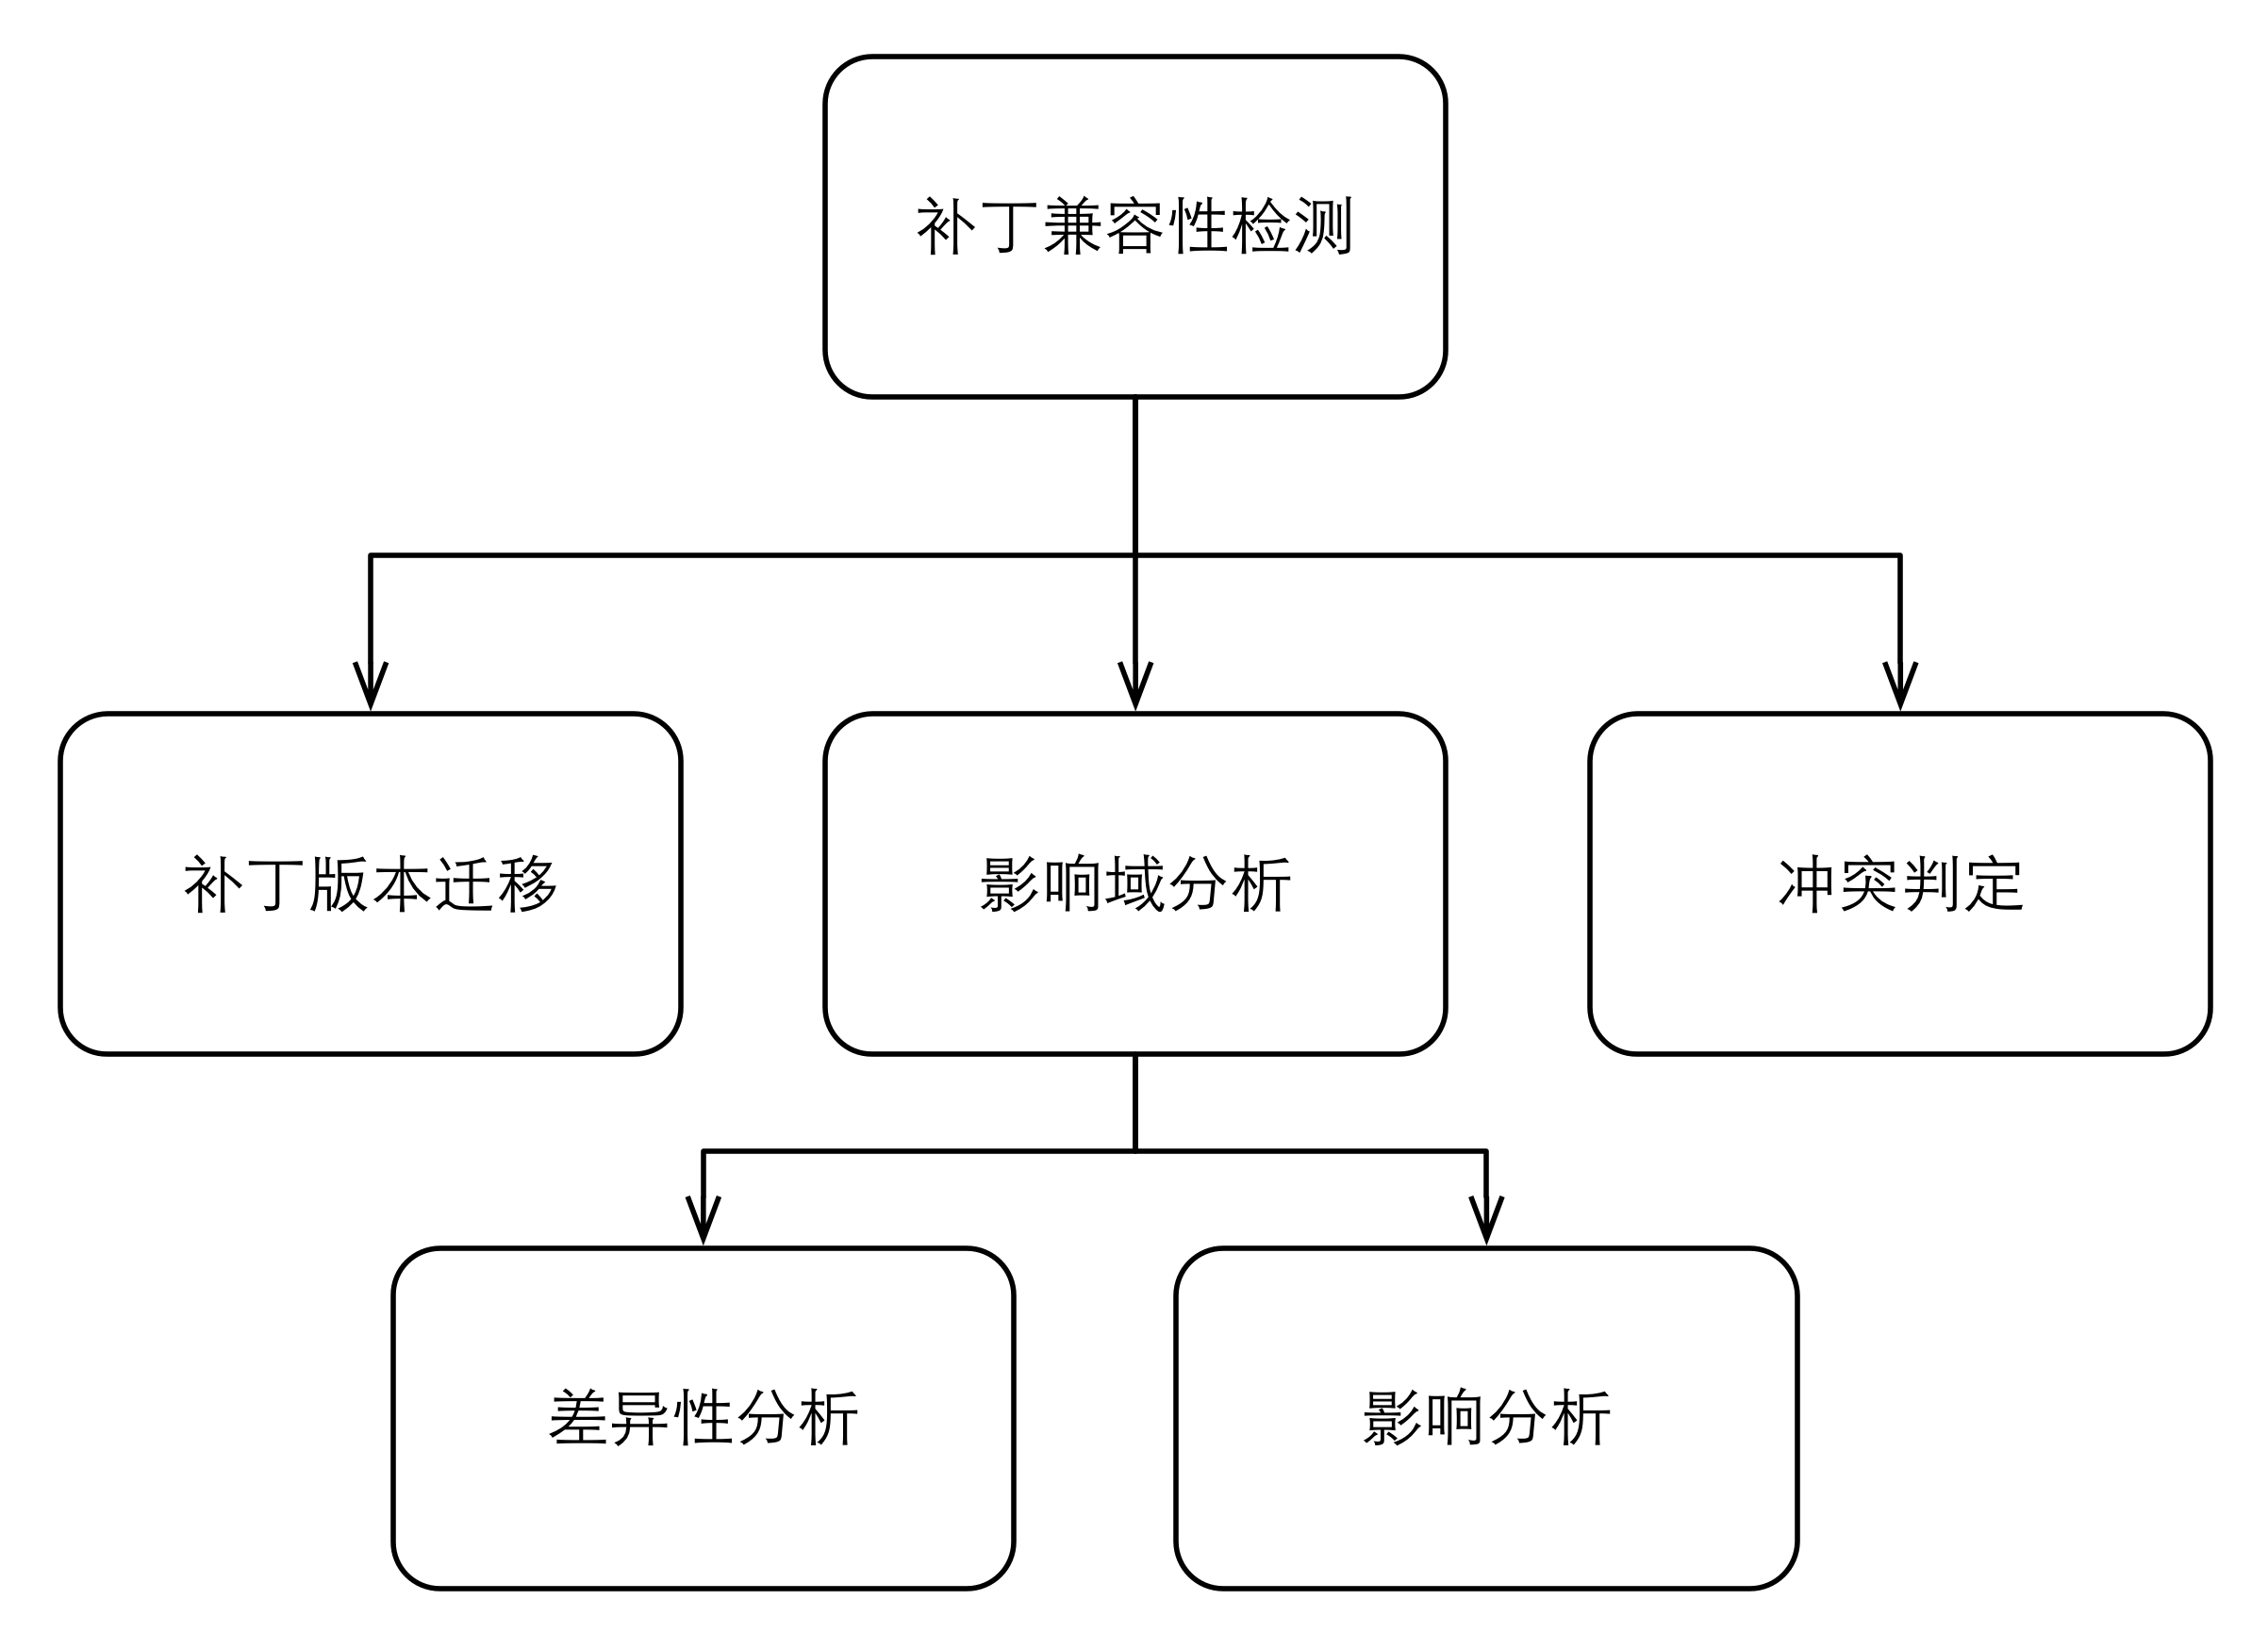
\includegraphics[height=.5\columnwidth]{chap03_structure}
	\caption {整体架构}	
	\label {structure}
\end{figure}

可见,兼容性检测工具可以拆分成三个模块:
\begin{itemize}
	\item 补丁版本迁移模块:实现解决方案中的补丁应用步骤。
	\item 影响域分析模块:实现解决方案中的软件变更影响域分析过程。
	\begin{itemize}
		\item 差异性分析模块:实现$diff$函数。
		\item 影响分析模块:实现$impact$函数。
	\end{itemize}
	\item 冲突判定模块:实现解决方案中的软件变更冲突检测方法。
\end{itemize}

整个工具的运作流程可以参考图\ref {solution_all}。其输入输出可以参考表\ref {all_io2}。

\begin{figure}[H]
	\centering
	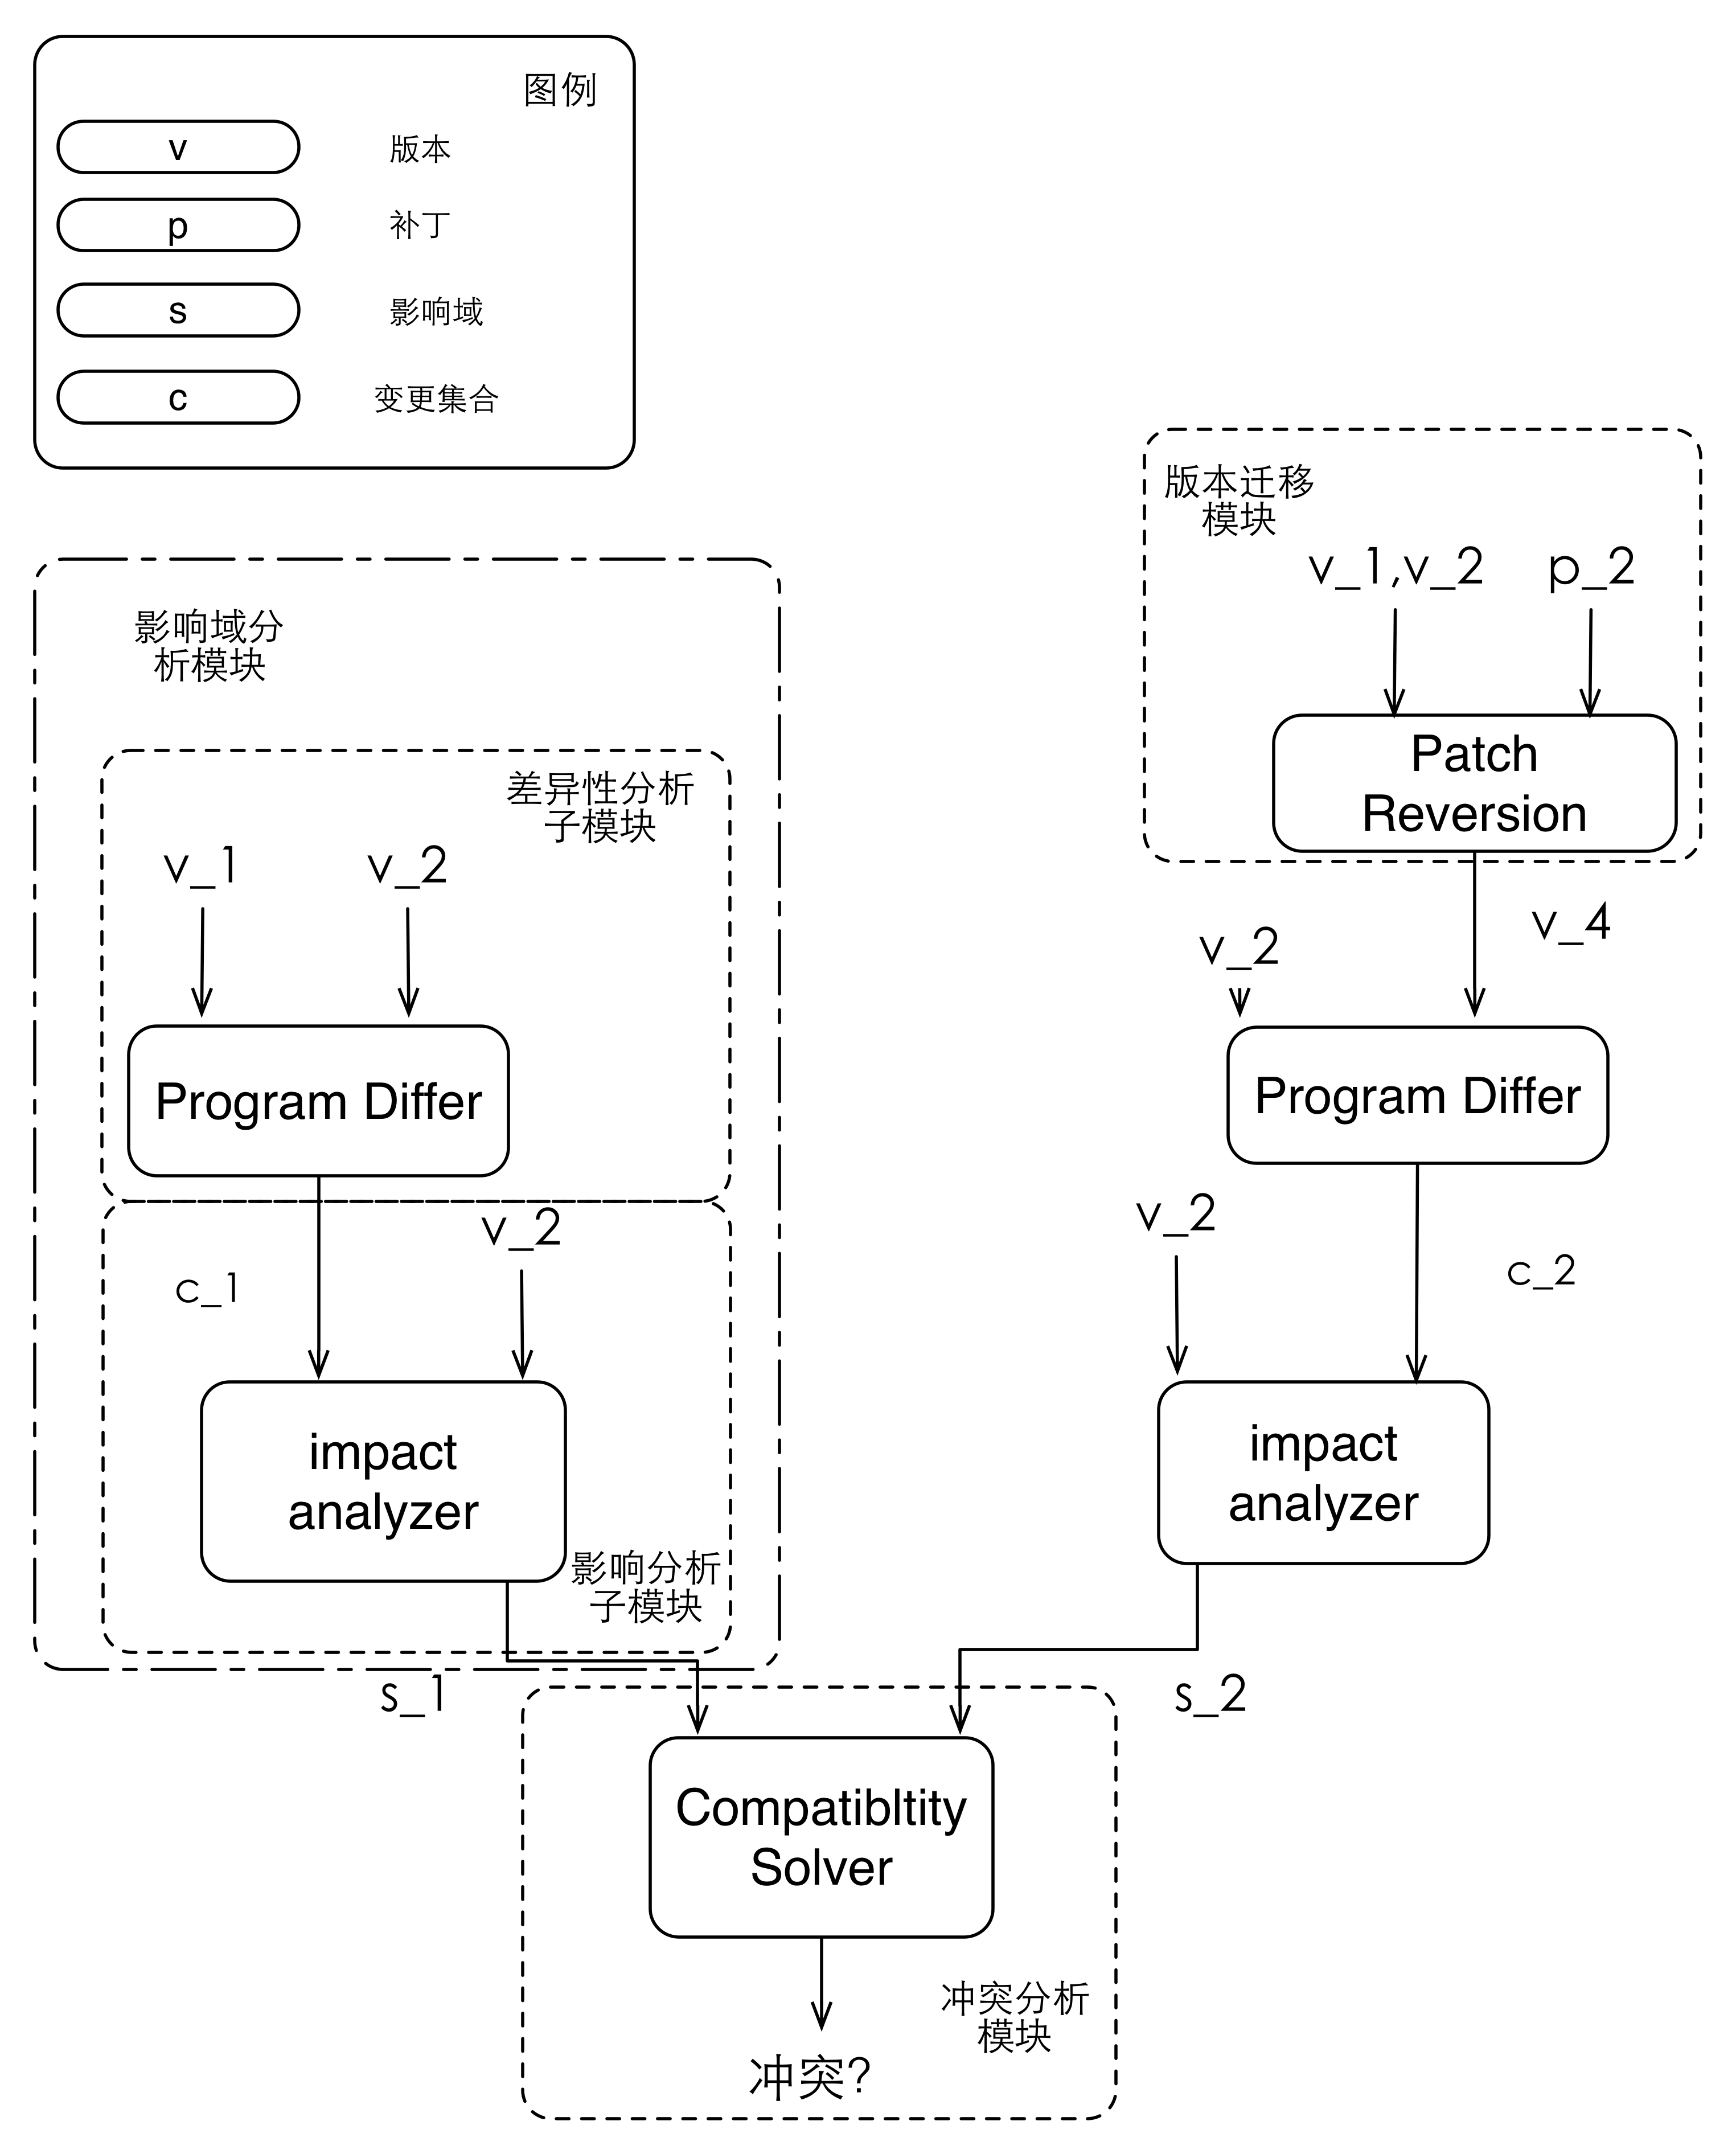
\includegraphics[width=.8\columnwidth]{chap03_all}
	\caption {工具流程}
	\label {solution_all}	
\end{figure}

\begin{table}[H]
	\caption{输入输出对照表}
	\label{all_io2}
	\centering
	\begin{tabular}{lc}
		\toprule[1.5pt]
		{\heiti 输入输出} & {\heiti 描述}\\\midrule[1pt]
		$v_1$ & 旧版本源代码,待检测的对象 \\
		$v_2$ & 新版本源代码 \\
		$v_4$ & 将补丁$p_2$中的变更应用于版本$v_1$后的源代码 \\
		$p_2$ & 适用于$v_2$的补丁,待检测的对象 \\
		$p_1$ & 补丁,版本$v_1$和$v_2$之间的变更集合\\
		$p_3$ & 补丁,版本$v_4$和$v_2$之间的变更集合\\
		$s_1$ & 变更集合$p_1$对版本$v_2$的影响域 \\
		$s_2$ & 变更集合$p_3$对版本$v_2$的影响域 \\
		结果 & 是否冲突\\
		\bottomrule[1.5pt]
	\end{tabular}
\end{table}

其工作流程可以简述如下:

\begin{enumerate}
	\item 采用版本控制系统进行代码版本管理,并进行补丁版本迁移,得到应用于新版本的补丁后代码版本$v_4$。
	\item 根据得到的三个版本代码$v_1$、$v_2$、$v_4$,分别分析其程序间差异性,生成对应的程序变更集合。
	\item 根据得到的程序变更集合,进行不同版本间的变更影响分析,生成语义影响域。
	\item 根据得到的语义影响域,进行冲突分析。
\end{enumerate}

\subsection{方法概述}

%如章节\ref {patch_app}中所述,我们可以采用常见的版本控制工具提供的三路归并算法进行补丁的版本迁移工作。具体来讲,其流程可以简述如下:
%\begin{enumerate}
%	\item 将补丁$p_1$应用到版本$v_1$,获得旧版本应用补丁后的代码,即其版本为$v_3 = patch(p_1,v_1)$。
%	\item 采用三路归并算法实现$v_4 = merge(v_2,v_3)$过程,获得新版本应用补丁后的代码$v_4$。
%	\item 解决分支合并中可能出现的冲突问题。
%\end{enumerate}

%其中,通过三路归并算法进行的合并工作中可能会出现冲突,这说明版本$v_2$和$v_3$之间存在语法冲突,即这两个版本在语法层面上不兼容。我们可以通过人工修改的方式进行修复,实现语法层面上的兼容性。

本节中主要对补丁兼容性检测方法进行概述,并说明方法中各步骤的目的。

如前所述,兼容性检测方法的第一步是进行补丁版本迁移,该过程即为$merge$函数的具体实现,它是为了将专为某个特定版本而设计的补丁应用于其他版本,并且消除该过程中可能产生的语法错误。

该步骤对应检测工具中的版本迁移模块,在实现中采用git工具的三路归并算法完成。具体来讲,其流程可以简述如下:
\begin{enumerate}
	\item 将补丁$p_1$应用到版本$v_1$,获得旧版本应用补丁后的代码,即其版本为$v_3 = patch(p_1,v_1)$。
	\item 采用三路归并算法实现$v_4 = merge(v_2,v_3)$过程,获得新版本应用补丁后的代码$v_4$。
	\item 解决分支合并中可能出现的冲突问题。
\end{enumerate}

其中,通过三路归并算法进行的合并工作中可能会出现冲突,这说明版本$v_2$和$v_3$之间存在语法冲突,即这两个版本在语法层面上不兼容。在该模块的具体实现中,我们可以使用第三方的合并工具Beyond Compare解决冲突,以实现语法层面上的兼容性。

%该补丁应用的过程主要用于解决补丁的版本适应性问题,整个过程可以用算法\ref {algo_patch}描述如下。
%
%\begin{algorithm}[H]
%	\caption{补丁应用}
%	\label{algo_patch}
%	\begin{algorithmic}[1]
%		\Require $v_1,v_2,p_1$
%		\Ensure $v_4$
%		\State $v_3 \gets patch(p_1,v_1)$
%		\State $v_4 \gets merge(v_2,v_3)$
%		\State $v_4 \gets resolve(v_4)$
%		\State\Return{$v_4$}
%		\State
%		\Function {merge}{$new,old\_patched$} 
%			\State\Return{$3-way-merge(old,new,old_patched)$}
%		\EndFunction
%		\State
%		\Function {resolve}{$version$} 
%			\State\Return{$mergetool(version)$}
%		\EndFunction		
%	\end{algorithmic}
%\end{algorithm}

%\subsection{语义影响域分析}
%\label {sia}

检测方法的第二个步骤是软件变更影响域分析的过程。通过该过程,我们能够找到两个补丁中的变更集合所对应的影响域,该影响域划定了变更集合对于其他程序代码结构的影响范围。

实际上,语义影响域分析主要分为两个分析过程,即程序间差异分析和变更影响分析,通过这两个分析的协作来完成整个语义影响域的分析。这两个子过程即为$diff$和$impact$函数的具体实现。

变更影响域分析所对应的工具模块是影响域分析模块,该模块在实际实现过程中也同样划分为两个子模块:
\begin{itemize}
	\item 差异性分析模块:该模块采用ASTro工具来实现具体的程序差异性分析算法。
	\item 影响分析模块:该模块采用jpf-regression工具来实现具体的变更影响分析算法。
\end{itemize}

在具体的模块实现过程中,我们发现一些主要需要解决的问题包括:
\begin{enumerate}
	\item 修正ASTro的分析结果,以提高精确度。
	\item 改进jpf-regression工具,包括:
	\begin{enumerate}
		\item 修复工具中自带的Bug。
		\item 修改工具的分析过程。
		\item 增加影响追踪系统。
		\item 增加错误记录系统。
	\end{enumerate}
	
	\item 实现实验过程的批量化和自动化。
\end{enumerate}

详细的影响域分析方法介绍与实现将在第\ref {chap_impact}章中给出。

%
%\subsubsection{程序差异性分析}
%
%程序差异性分析是$diff$函数的实现。它主要用于分析两个不同版本的程序间的差异性,其结果即我们所需要的程序变更集合。近年来程序差异性分析方面有不少工作,实现了一些较为成熟的比较工具,我们可以使用这些工具来实现该分析过程。
%
%在本文的组合架构中,程序差异性分析的主要任务是接受两个不同版本的源代码,并返回代码间的结构化差异信息。结构化的差异信息可以视为补丁的一种,只不过它具有比常见的采用Unix diff工具生成的$.patch$类型的补丁文件更丰富的信息,能够描述以程序语法结构的形式对软件变更进行描述。
%
%该分析过程应该满足如下需要:
%\begin{itemize}
%	\item 输入为两个不同版本的代码。
%	\item 输出为源代码间的软件变更集合。
%	\item 每条变更描述语句或基本块级别的变更。
%	\item 每条变更描述新旧程序结构的相关信息和其关联关系。
%	\item 每条变更描述了其所属的作用域。
%\end{itemize}
%
%选择这样的分析结果类型是为了后续分析过程的方便,因为变更影响分析需要我们提供软件变更集合作为输入,而$.patch$类型的补丁文件只描述文本行的变更,不包含语法信息,我们无法从中提取出所需的语法层面的变更信息。
%
%一种比较好的选择是采用AST差异性分析,因为抽象语法树中包括了足够多的语法结构信息。
%
%
%
%%图中所描述的软件变更集合可以定义如下:
%%\begin{definition}
%%	$ change\_set = \{ (old_i,new_i) \mid  old_i \subset Structure,new_i \subset Structure, i \subset \mathbb{N} \}$
%%\end{definition}
%
%
%
%\subsubsection{变更影响分析}
%
%程序变更影响分析是$impact$函数的具体实现。主要用于获取变更集合对其他程序结构的影响域,该集合所包含的程序结构直接或间接地受到变更集合中的元素影响。近年来这方面比较成熟的工作也有不少,因而可以直接选择合适的变更影响分析算法作为该过分析过程的具体实现。
%
%在本文的组合架构中,该分析过程应当接受两个不同版本代码间的变更集合作为输入,并输出变更集合所对应的影响集合,这也就是我们所需要的变更集合的语义影响域。变更影响分析的过程可以通过控制流、数据流等信息分析出变更集合中每条变更对其他程序结构是否存在影响,并进行闭包计算即可。
%
%本文对于该分析过程的要求如下:
%\begin{itemize}
%	\item 接受两个不同版本代码间的变更集合作为输入。
%	\item 计算得到该变更集合所对应的影响集合。
%	\item 计算过程中可以指定受影响的范围和元素类型。
%	\item 影响集合中的元素按照其不同类型进行分类。
%	\item 具有影响追踪系统,将计算影响域的过程进行记录。方便后续的冲突分析过程进行回溯。
%\end{itemize}
%
%其中影响追踪系统可以定义成如下类型的函数。该函数接受一个影响域分析函数$ia(v_i,v_j)$,并返回对应的依赖关系集合。
%
%\begin{definition}
%	$impact\_track(ia(v_i,v_j)):(Code \times Code \mapsto {Structure}) \mapsto {depend}$
%\end{definition}
%
%
%%该分析过程如图\ref {impact_analyzer}所述,其中的$impact$函数可以任意选择某一能够满足上述要求的变更影响分析算法。
%%
%%图中所描述的变更影响集合可以定义如下:
%%\begin{definition}
%%	$impact\_set = \{ (structure_i) \mid  structure_i \subset Structure, i \subset \mathbb{N}\}$
%%\end{definition}
%%
%%\begin{figure}[H]
%%	\centering
%%	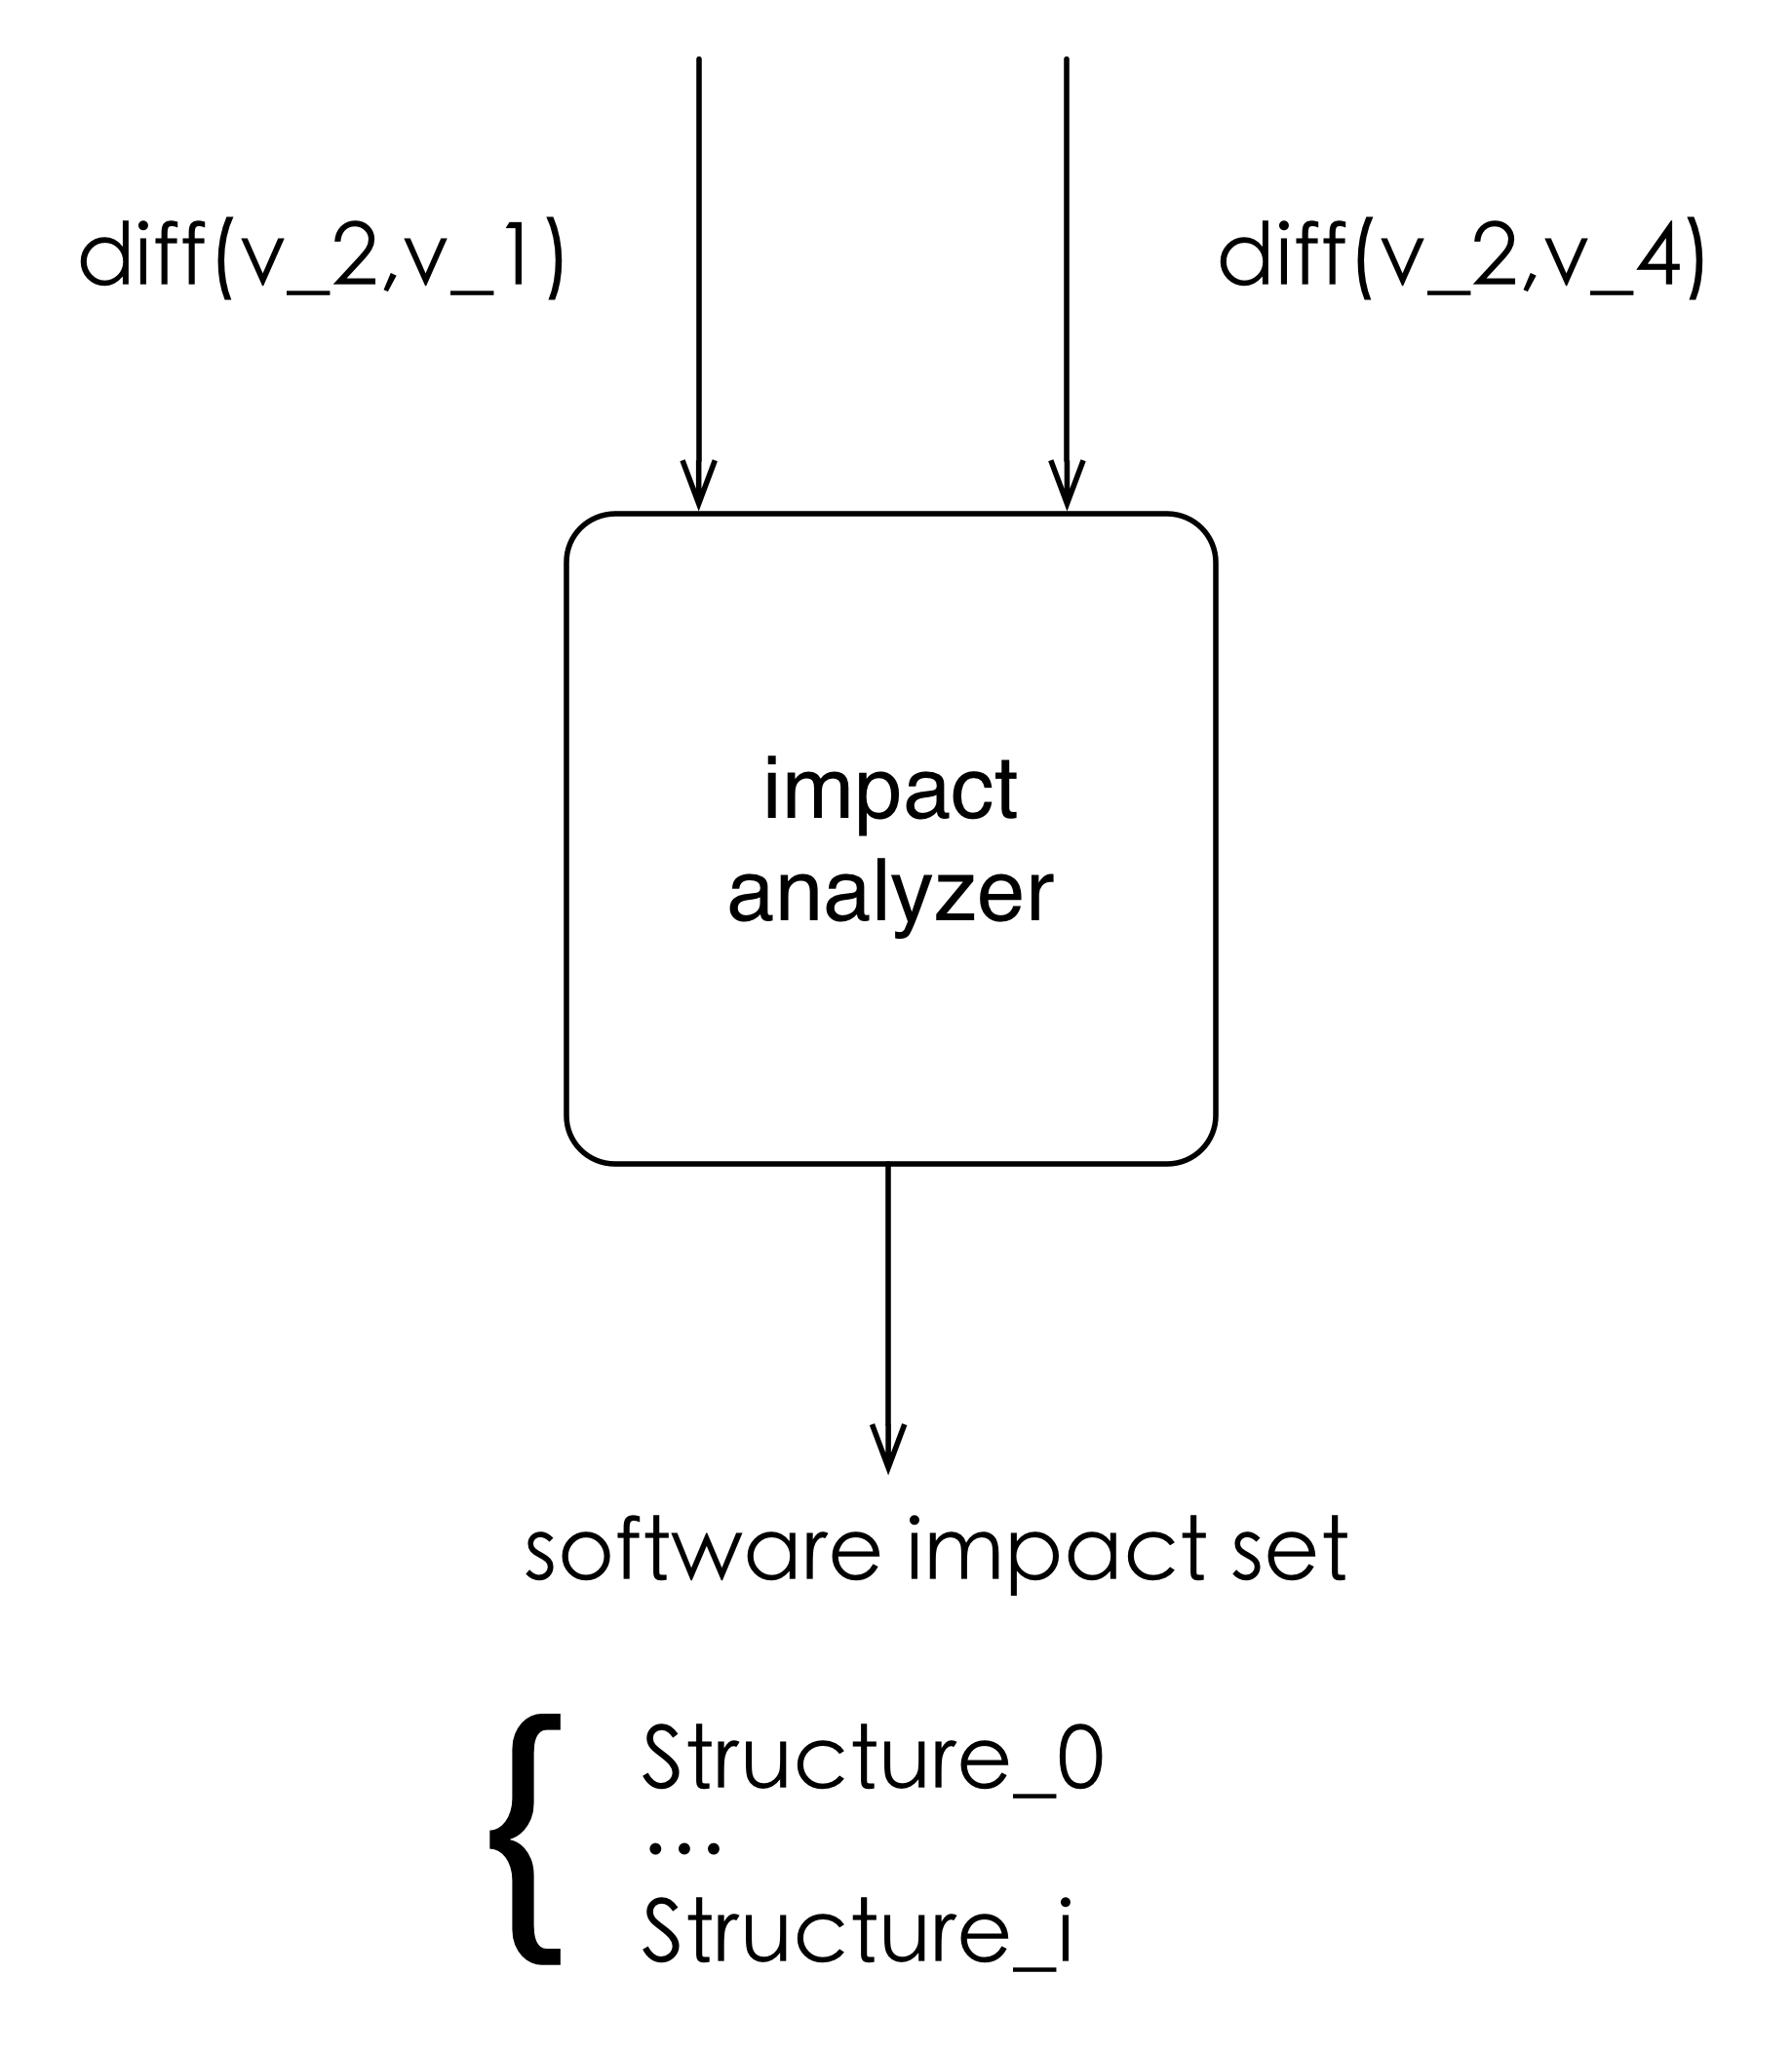
\includegraphics{chap03_impact}
%%	\caption {程序间差异分析}
%%	\label {impact_analyzer}	
%%\end{figure}
%
%在完成了上述两项子分析过程后,我们就完成了整个语义影响域分析过程,并获得了两个不同版本代码的变更集合和对应的其语义影响范围。接下来就可以进行具体的兼容性分析工作。
%
%整个语义影响域分析过程可以用算法\ref {algo_impact}描述。
%
%\begin{algorithm}[H]
%	\caption{语义影响域分析算法}
%	\label{algo_impact}
%	\begin{algorithmic}[1]
%		\Require $v_i,v_j$	
%		\Ensure $s$
%		\Function {ia}{$v_i,v_j$}
%			\State $p \gets diff(v_i,v_j)$
%			\State $s \gets impact(p,v_i)$
%			\State\Return{$s$}
%		\EndFunction
%	\end{algorithmic}
%\end{algorithm}

%\subsection{冲突分析}

检测方法的第三步为软件变更冲突检测方法,该过程即为$conflict$函数的具体实现。我们将对比两个补丁的变更影响域,判定他们是否重叠,并以此为依据找到可能发生冲突的代码位置。更精确的冲突判定过程需要人工分析的辅助。

冲突检测方法对应工具中的冲突判定模块,该模块实现了具体的冲突检测算法,它将接收影响域分析模块的输出,并分析并找到变更影响域间的重叠。

详细的冲突检测方法介绍与实现可以参考第\ref {chap_conflict}章。
%
%理论上来讲,这种简单比对即可发现两个版本间的兼容性问题,因为一旦发生重叠,那么重叠的代码部分显然是会发生兼容性问题的。然而在实际情况中,受限于工具的精度,我们往往不能达到理论上的准确度,而可能会发生误报(False Negative)等情况。
%
%显然,如果重叠不存在,则兼容性是可以得到满足的。而对于如何界定重叠部分的兼容性,则需要人工分析的介入,因为这部分代码的兼容性与补丁的功能目标密切相关,而我们无法从代码中获取到这种信息,因而只有依靠外界来提供,并以此为依据进行详细分析过程,界定这部分代码是否真的存在冲突。
%
%在进行人工分析的过程中,我们不仅需要知道哪部分代码出现了重叠现象,而且还需要知道是哪些变更影响到了这部分代码,因而我们需要引入影响追踪系统来记录变更影响分析过程的轨迹。影响追踪系统可以记录下变更影响分析过程中的每一步,从而获取到程序结构间的影响关系链,事后通过回溯即可追踪到具体的软件变更可见,本过程中主要需要影响追踪系统的回溯模块的支持。

%可以看得出来,由于使用了更严格的冲突定义,我们的方法会造成一定的过高估计的结果。

%该分析过程可以参考算法\ref {algo_compatible}。
%
%\begin{algorithm}[H]
%	\caption{冲突分析}
%	\label{algo_compatible}
%	\begin{algorithmic}[1]
%		\Require $s_1=ia(v_2,v_1)$,$s_2=ia(v_2,v_4)$\\
%				 \quad \quad $t_1=impact\_track(ia(v_2,v_1))$, $t_2=impact\_track(ia(v_2,v_4))$
%		\Ensure $isCompatible(diff(v_2,v_1), diff(v_2,v_4))$
%		\If{$s_1 = \varnothing \lor s_2 = \varnothing$}
%			\State $result \gets True$
%		\Else
%			\State $s \gets s_1 \cap s_2$
%			\If{$s = \varnothing$}
%				\State $result \gets True$
%			\Else				
%				\State $result \gets Manual\_analysis(s_1, s_2, t_1, t_2)$
%			\EndIf 
%		\EndIf
%		\Return $result$
%	\end{algorithmic}
%\end{algorithm}

%整个分析过程的架构如图\ref {isCompatible}所示。
%
%\begin{figure}
%	\centering
%	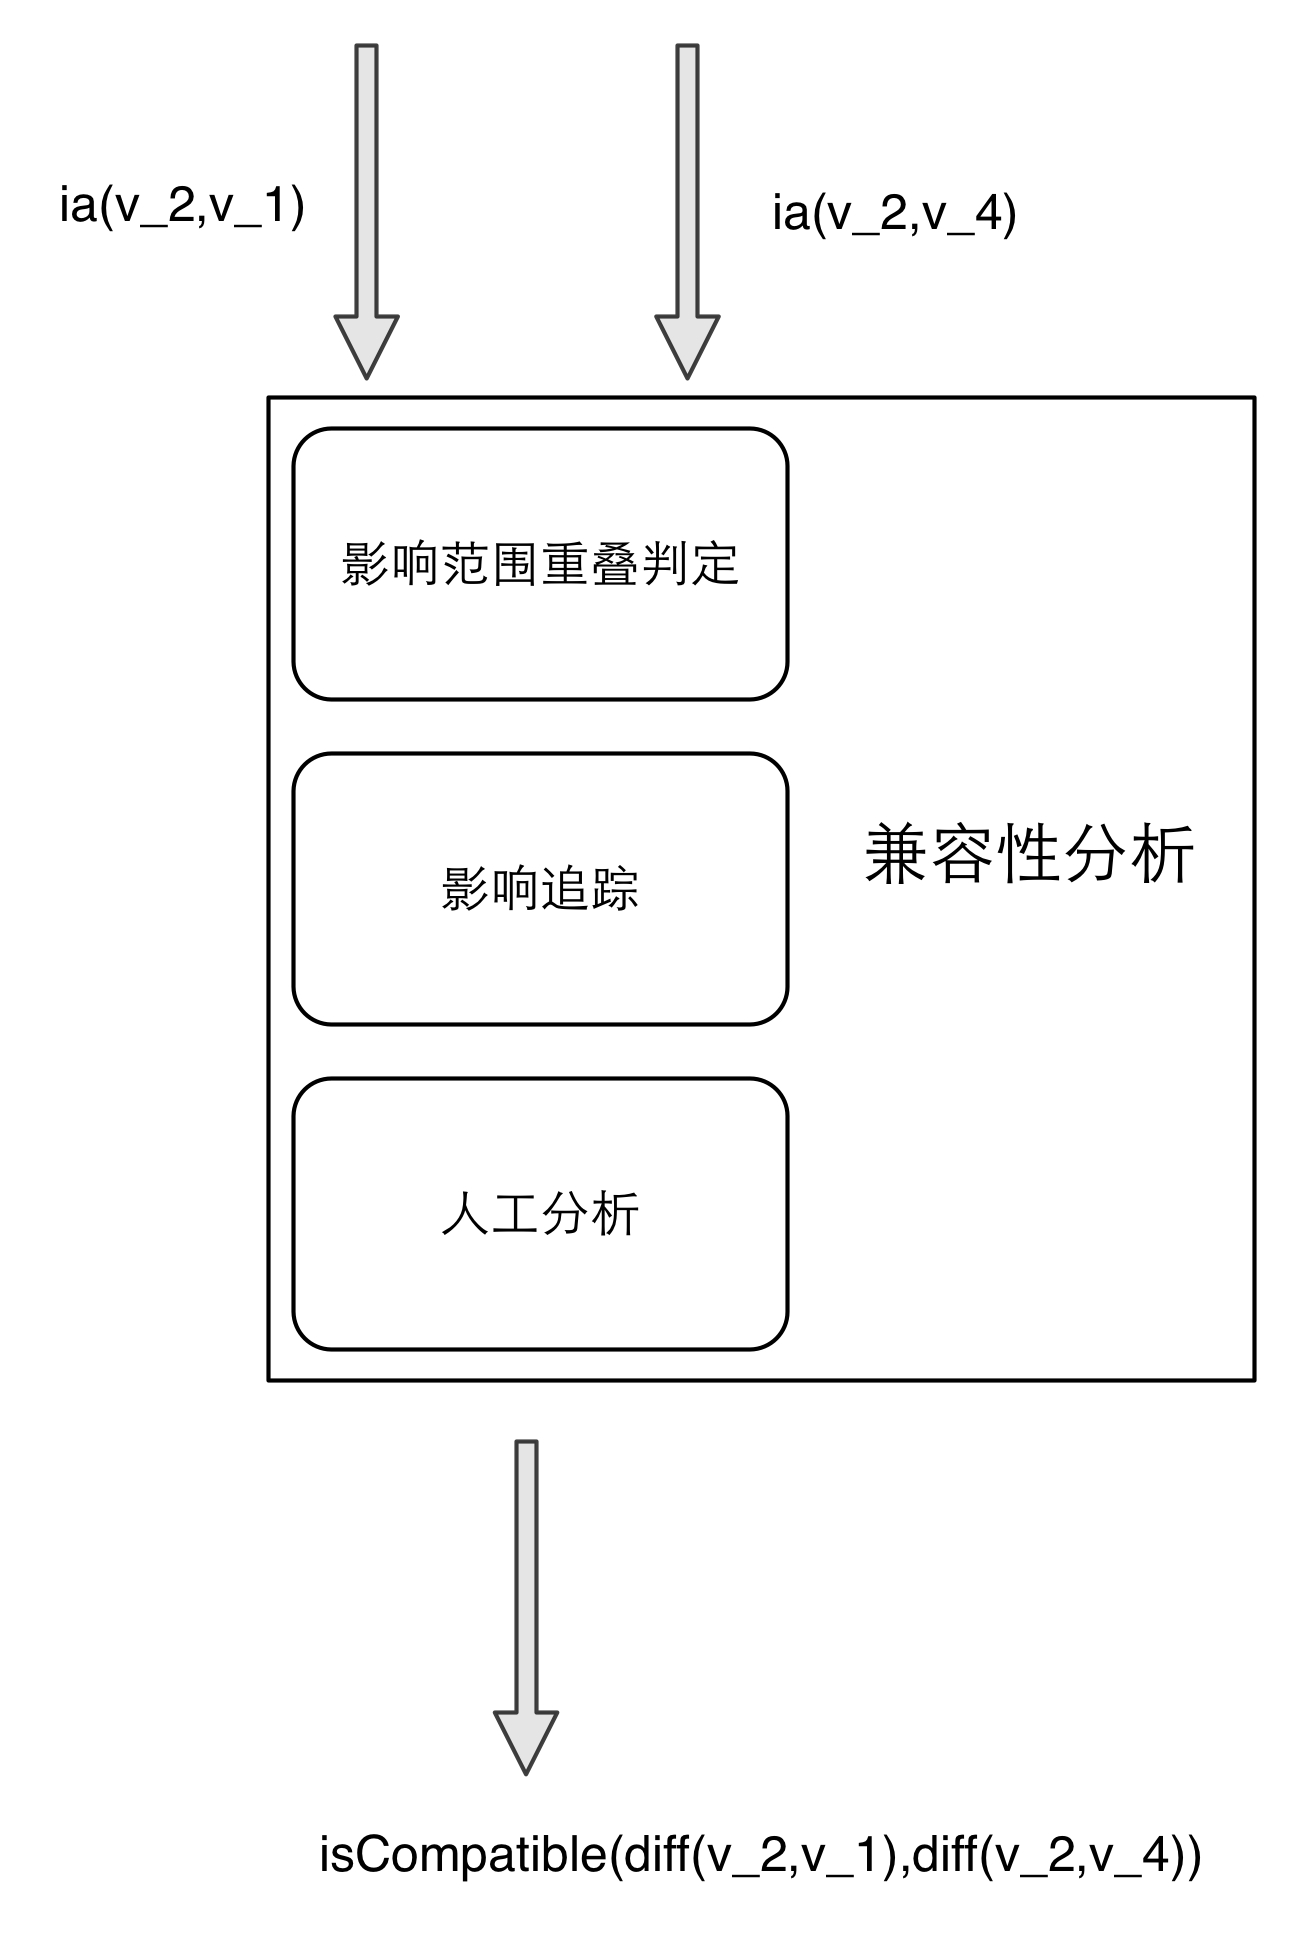
\includegraphics{chap03_isCompatible}
%	\caption {兼容性分析}
%	\label {isCompatible}	
%\end{figure}


\section{本章小结}
本章主要介绍了软件补丁兼容性检测所关注的主要问题以及如何解决该问题。

章节\ref {define_problem}中对兼容性问题进行了定义和分析。

章节\ref {problem_solve}根据将前一节中提到的分析方法,提出了一套通用的兼容性检测方法和对应的工具实现,并简要介绍了其中涉及的方法。